%%%%%%%%%%%%%%%%%%%%%%%%%%%%%%%%%%%%%%%%%%%%%%%%%%%%%%%%%%%%%%%%%%%%%%%%%%%%%%%%
% reconstruction.tex:
%%%%%%%%%%%%%%%%%%%%%%%%%%%%%%%%%%%%%%%%%%%%%%%%%%%%%%%%%%%%%%%%%%%%%%%%%%%%%%%%
\chapter{Event Reconstruction}
\label{sec:reco_chapter}
%%%%%%%%%%%%%%%%%%%%%%%%%%%%%%%%%%%%%%%%%%%%%%%%%%%%%%%%%%%%%%%%%%%%%%%%%%%%%%%%

Electrons, muons and jets expected from \WR and \nul decays traverse multiple CMS sub-detectors, as shown in 
Figure \ref{fig:particleTrajectories}.  Their trajectories and energies were measured from charged particle tracks 
reconstructed by the silicon tracker and muon detectors, and energy deposits reconstructed by the calorimeters.  The 
high energy of expected leptons and jets motivated the use of specific lepton and jet reconstruction algorithms 
described here.  These algorithms combine measurements from multiple CMS sub-detectors to measure the trajectory 
and energy of each particle with the best resolution.  For charged particles, initial energy and trajectory 
measurements are made using tracks reconstructed from signals measured in the silicon tracker.

\begin{figure}[h]
	\centering
	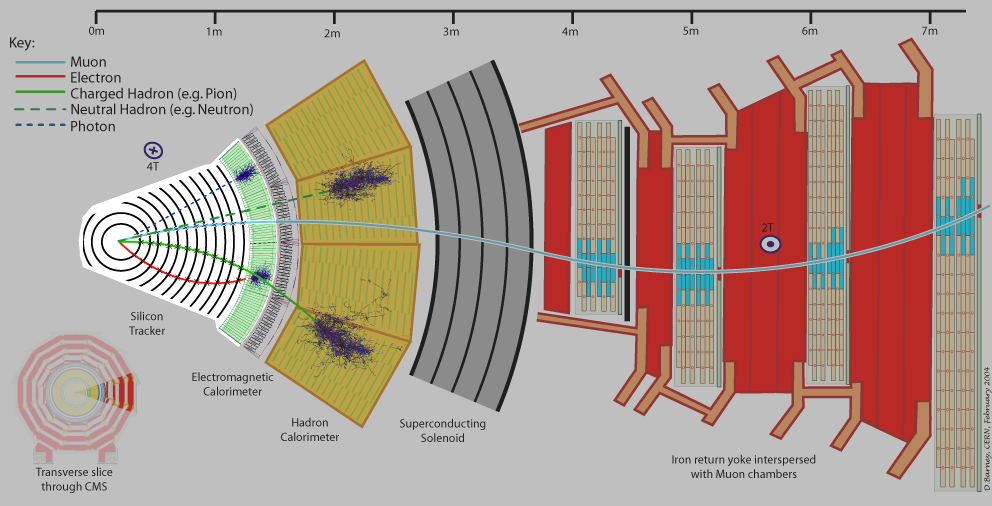
\includegraphics[width=0.75\textwidth]{figures/flowOfParticlesThroughCMS.png}
	\caption{Typical trajectories of particles travelling through CMS, from CERN.}
	\label{fig:particleTrajectories}
\end{figure}


\section{Track Reconstruction}
\label{sec:trkReco}
Charged particles are reconstructed as helical tracks from signals measured in the silicon tracker.  An interative algorithm 
starts by reconstructing tracks from signals in the inner pixel tracker characterized by the highest energies or smallest 
distances from the IP, and progressively includes signals measured in outer pixel tracker and silicon strip tracker layers.  
Signals in successive layers are linked into continuous tracks using a Kalman filter that requires each signal to have 
$\chi^{2} <$ 30 \cite{trackerPerformanceInCollisions}.  Each time a new signal is added to a track, an analytic function 
extrapolates the track trajectory to the next layer assuming energy is lost only through ionization in the silicon.  Hits in 
the next layer are searched for in the region identified by the analytic function extrapolation, and this procedure repeats 
until signals are included from the outermost silicon strip tracker layer.  Then, the signals linked into tracks are removed 
from the list of track candidates, and the algorithm restarts using signals measured in the inner pixel tracker characterized 
by lower energies or larger distances from the IP.  Using this algorithm, isolated muons with $\pt > 0.9$ $\GeV$ and $|\eta| < 2.4$ 
were reconstructed as tracks with essentially 100\% efficiency \cite{trackerPerformanceInCollisions}.  After reconstructing 
all tracks in an event, each point where two or more tracks originate is identified as an interaction vertex, and its position 
is measured relative to the IP.  The positions of vertices that have muon tracks with $|\eta| < 1.4$ and $\pt = 100$ $\GeV$ 
were measured with 10 and 30 $\mu$m resolutions in the transverse (r-$\phi$) and longitudinal ($z$) directions.

The track reconstruction algorithm described previously is used to reconstruct muon and charged hadron tracks, but a second 
algorithm is used to reconstruct electron tracks.  The silicon tracker contains, depending on $\eta$, 1 to 2 radiation 
lengths of material that causes electrons to shower.  As a result, $\sim$35\% of electrons that traverse the tracker lose more 
than 70\% of their initial energies through bremsstrahlung \cite{trackerPerformanceInCollisions}, which cannot be measured by 
the tracker.  The electron track reconstruction algorithm uses the same iterative track reconstruction procedure described 
previously, but extrapolates each track's trajectory to the next silicon layer assuming the energy lost through bremsstrahlung 
is described by a sum of Gaussians.  In addition, the Kalman filter used to link signals in successive layers requires that new 
signals have $\chi^{2} <$ 2000.  The electron track algorithm reconstructed electrons with $\pt > 20$ $\GeV$ and $|\eta| < 2.5$ 
as tracks with 97\% or better efficiency \cite{gsfPerformanceInCollisions}.


\section{Energy Reconstruction}
\label{sec:enrgReco}
The energies of photons, electrons, and hadrons produced by pp interactions are measured in groups of ECAL crystals.  Photons, 
electrons, and hadrons impinging on the ECAL generate signals in the ECAL crystals that are converted into uncalibrated energies.  Groups, 
or superclusters (SCs), of crystals are built from the most energetic crystals with $\Et \gtrsim 0.2$ $\GeV$ and their nearest 
neighbors, and are at least 3 crystals wide in $\eta$.  The upstream tracker material causes $\sim$35\% of electrons and 
photons, and up to 25\% of hadrons \cite{trackerPerformanceInCollisions} to shower in the tracker, and radiate energy by emitting 
photons and other particles.  The energy is typically radiated along the particle's $\eta$ trajectory, but spread over several ECAL 
crystals in $\phi$.  To capture this energy, each SC is at least 5 crystals wide in $\phi$, and can be much larger, 
as shown in Figure \ref{fig:eleTrackAndSC}.  Once a SC is built, the energy of each crystal in the SC is multiplied by a laser 
transparency correction, and relative and absolute energy calibration corrections.  The sum of the calibrated crystal energies 
is the SC energy, and the energy weighted average $(\eta,\phi)$ position is the SC position.  Using only ECAL SCs, the $(\eta,\phi)$ 
positions of electrons in the barrel (endcap) were measured with a $\phi$ resolution of 0.17$^{\circ}$ (0.29$^{\circ}$), and an 
$\eta$ resolution of 0.001 (0.002) units.

The energies of hadrons that traverse the ECAL are measured in groups of HCAL towers.  Hadrons impinging on the HCAL generate signals 
in the HCAL towers that are converted into uncalibrated energies.  The highest energy towers with $\Et \gtrsim 1$ $\GeV$ are used to 
seed clusters, which extend to all neighboring towers with $\Et > 0.8$ $\GeV$ \cite{pflowEventReco}.  If one tower is grouped into 
multiple clusters, the tower's contribution to each cluster is weighted by its distance from each cluster's seed.  After clusters are 
built, each tower's energy is multiplied by a laser transparency correction, and relative and absolute energy calibration corrections.  
The sum of the calibrated tower energies is the cluster energy, and the energy weighted average $(\eta,\phi)$ position is the cluster 
position.  Hadron energies are measured as a combination of calibrated HCAL cluster energies, and energies of overlapping ECAL SCs.  
Using the combined ECAL-HCAL system, hadrons with $\Et = 100$ $\GeV$ were measured with a $\sim$10\% $\Et$ resolution \cite{pflowEventReco}.


\section{Muon Reconstruction}
\label{sec:muReco}
Muons are first reconstructed as tracks from signals measured in individual muon chambers.  In each DT chamber, the start and end points of 
track segments are identified first as pairs of signals measured in the same plane (r-$\phi$ or r-z) but in different layers.  Then straight 
lines are drawn between the signal pairs, and a signal pair is ignored if its line is not compatible with a track that extrapolates from 
the chamber to the IP.  The remaining signals that are consistent with any of these straight lines are built into track segments that are 
measured in at least 3 layers.  In each plane the track segment with signals in the largest number of layers, at least 3, and the lowest 
$\chi^{2}/nDOF$, less than 20, is used to build a 3D track.  In the event where more than one track segment is reconstructed 
in one plane of a DT chamber, all combinations of r-$\phi$ and r-z track segments are considered when reconstructing a 3D track.  In 
practice, more than one 3D track is reconstructed in a DT chamber in less than 1\% of events \cite{cmsTdrPhysPerformance}.  The same 
track segment reconstruction algorithm is used in each 6 layer, single plane CSC.  There the final track segment must have signals 
in at least 4 layers.  In the barrel-endcap transition region, $1.3 < |\eta| < 1.6$, where the DT chambers stop and the CSCs begin, RPCs 
are used to improve the muon reconstruction efficiency and the precision of arrival time measurements.  Each RPC contains two parallel 
plates divided into many thin strips, and strips that measure a signal are grouped into clusters.  Each reconstructed cluster represents 
a hit whose position is the 'center of gravity' of all the strips in the cluster.

Tracks reconstructed in individual chambers are used to reconstruct muon trajectories through the magnetic field and all muon chambers.  
A Kalman filter algorithm starts with tracks in the chambers closest to the IP, and predicts the track positions in chambers in the next 
radial station with the effects of an inhomogeneous magnetic field and material losses taken into account \cite{muonRecoFirstCollisions}.  
Track segments in outer chambers are added to existing tracks subject to a $\chi^{2}$ requirement, and existing tracks are propagated to 
the next radial station even if no matching track segment is found in the current station.  Once the outermost station is included, a 
reverse Kalman filter is applied to reconstructed tracks from the outermost station working to the innermost station.  The reverse Kalman 
filter finalizes the track parameters, then these tracks are compared to silicon tracker tracks to identify global muons.

Global muons are identified using tracks reconstructed in the silicon tracker and muon detectors.  Tracks from the muon detectors are 
extrapolated back to the outermost silicon tracker layer, and their positions are compared.  In the local coordinate plane of the 
silicon strip layer, each silicon tracker track that matches a muon detector track within 3 cm is identified as a global muon.  If an 
extrapolated muon detector track has multiple silicon tracker track candidates within 3 cm, the closest match is used to make a global 
muon.  The $(\eta,\phi)$ trajectory of each global muon corresponds to that of its silicon tracker track.

The momentum of each global muon is determined by sampling four different global muon reconstruction algorithms, and selecting the  
highest quality result.  Each algorithm fits a continuous track \cite{cmsMuonRecoRunTwo} to a unique combination of silicon tracker 
and muon detector signals to estimate a muon's trajectory through CMS, as represented in Figure \ref{fig:particleTrajectories}.  The 
quality of each continuous track is identified by a fit uncertainty $\chi^{2}/nDOF$ and momentum uncertainty $\sigma(\pt)/\pt$; and 
the track with the lowest $\chi^{2}/nDOF$ and momentum uncertainty $\sigma(\pt)/\pt < 0.3$ determines the global muon's momentum.  
For muons with $\pt \lesssim 100$ $\GeV$ the highest quality result is obtained using only silicon tracker measurements.  Muons with 
$|\eta| < 1.4$ and $\pt = 100$ $\GeV$ were measured with a $\pt$ resolution of $\sim$2.8\% \cite{trackerPerformanceInCollisions}.  
However, as a muon's $\pt$ increases above 100 $\GeV$ the silicon tracker $\pt$ resolution degrades faster that that of the muon 
detectors.  A significant fraction of $\WR \rightarrow \mu\mu jj$ events are expected to produce at least one muon with $\pt > 200$ $\GeV$ 
(Table \ref{tab:wrHighPtMuons}), and in this high $\pt$ region the highest quality momentum measurement is made by combining silicon 
tracker and muon detector measurements.  Muons with $|\eta| < 0.9$ and $200 < \pt < 400$ $\GeV$ were measured with a $\pt$ resolution 
of 3.2\%, and higher $\pt$ muons were measured with a resolution better than 6\% \cite{cmsMuonRecoRunTwo}.

\begin{table}[h]
	\caption{Fraction of expected $\WR \rightarrow \mu\mu jj$ events that had at least one muon with $\pt > 200$ $\GeV$. 
	($\mnul = \frac{1}{2}\mWR$)}
	\label{tab:wrHighPtMuons}
	\centering
	\begin{tabular}{c|c}
		\mWR ($\TeV$) & Fraction of events with at least one high-$\pt$ muon (\%) \\  \hline
		1.0 &  80.  \\
		2.0 &  95.  \\ 
		3.0 &  98.  \\ \hline
	\end{tabular}
\end{table}

Global muons reconstructed in simulated events are known to have different energies than muons reconstructed in data.  Energy 
corrections for simulated muons are derived using $Z \rightarrow \mu\mu$ events from simulations and data.  The di-muon mass 
($M_{\mu\mu}$) distribution in $Z \rightarrow \mu\mu$ events is compared between data and simulations, and the energies of muons 
in simulated events are corrected so that the two $M_{\mu\mu}$ distributions match.


\section{Electron Reconstruction}
\label{sec:eleReco}
Electrons are the only particles from \WR decays expected to lose more than a few percent of their initial energy through 
bremsstrahlung in the tracker.  A dedicated electron track reconstruction algorithm is used to reconstruct tracks from electrons, 
even those that experience large energy losses, with high efficiency, but the tracker cannot measure the magnitude of bremsstrahlung 
energy losses.  However, the energies of electrons and their bremsstrahlung photons are measured by the ECAL.  Therefore, the ECAL 
is used to measure the $\Et$ and $(\eta,\phi)$ trajectory of each electron.

Electrons are identified using reconstructed tracks and ECAL SCs.  Reconstructed tracks are extrapolated from the outermost 
silicon strip layer to the front face of the ECAL, and their positions are compared to ECAL SCs.  Each electron is identified 
as one or more tracks that match the SC $(\eta,\phi)$ position within 1.1$^{\circ}$, about 1 crystal wide, in $\phi$, and 
within 0.004 units, less than $\frac{1}{2}$ a crystal wide, in $\eta$.  In addition, the ECAL SC $\Et$ and the matched 
track $\pt$ must agree within the uncertainty on the track $\pt$.  Using the SC energy, electrons with $\Et \approx 45$ 
$\GeV$ and $|\eta| < 0.8$ were measured with an $\Et$ resolution better than 2\%, and a resolution between 2\% and 5\% 
for higher $|\eta|$ \cite{ecalPerformanceInCollisions}.

\begin{figure}[h]
	\centering
	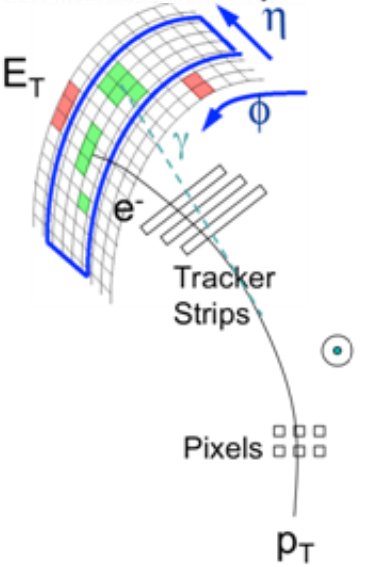
\includegraphics[width=0.75\textwidth]{figures/electronTrackAndSupercluster.png}
	\caption{The trajectory of a typical electron through the tracker and the ECAL.}
	\label{fig:eleTrackAndSC}
\end{figure}

Electrons reconstructed in simulated events are known to have different energies than electrons reconstructed in data.  Energy 
corrections for simulated electrons are derived using $Z \rightarrow ee$ events from simulations and data.  The di-electron mass 
($M_{ee}$) distribution in $Z \rightarrow ee$ events is compared between data and simulations, and the energies of electrons 
in simulated events are corrected so that the two $M_{ee}$ distributions match.


\section{Jet Reconstruction}
\label{sec:jetReco}
%On average, 85 percent of a jet's energy is carried by photons and charged particles  \cite{pflowJetRecoInCollisions}

%PF algo reconstructs muons first, then estimates the muon energy in ECAL and HCAL and subtracts this energy from 
%the calorimeter clusters.  The silicon tracker tracks associated with reco muons are removed from the list of charged particle candidates.
%then electrons are reconstructed, after which their tracks are removed from the list of candidates.
%lastly, photons and charged and neutral hadrons are reconstructed from the remaining calo energy clusters and tracks

%RESUME HERE

Through hadronization, photon radiation, and leptonic weak decays, quarks produced jets of photons, hadrons, and leptons.  
Thus, photons, electrons and muons, and charged and neutral hadrons were reconstructed before jets were built.  Photons 
were reconstructed in the ECAL as superclusters that did not overlap in $(\eta,\phi)$ with any energy deposits measured 
in the HCAL, and were separated from any reconstructed track by at least 1.1$^{\circ}$ in $\phi$ and 1 ECAL crystal in $\eta$.  
Charged and neutral hadrons were reconstructed in the HCAL as individual or multiple neighboring towers, and were 
reconstructed in the ECAL as superclusters that overlapped with the HCAL towers \cite{pflowJetRecoInCollisions}.  Each 
charged hadron was identified as a track, reconstructed as described for muons in Section \ref{sec:muReco}, that extrapolated 
to the $(\eta,\phi)$ area of the ECAL SC or at least one of the HCAL towers.  Each neutral hadron was identified as an HCAL 
energy cluster, and possibly an ECAL SC, that did not overlap with any reconstructed track in $(\eta,\phi)$.  After 
individual particles were reconstructed, jets were built from clusters of individual particles, as shown in Figure 
\ref{fig:jetClustering}.

\begin{figure}[h]
	\centering
	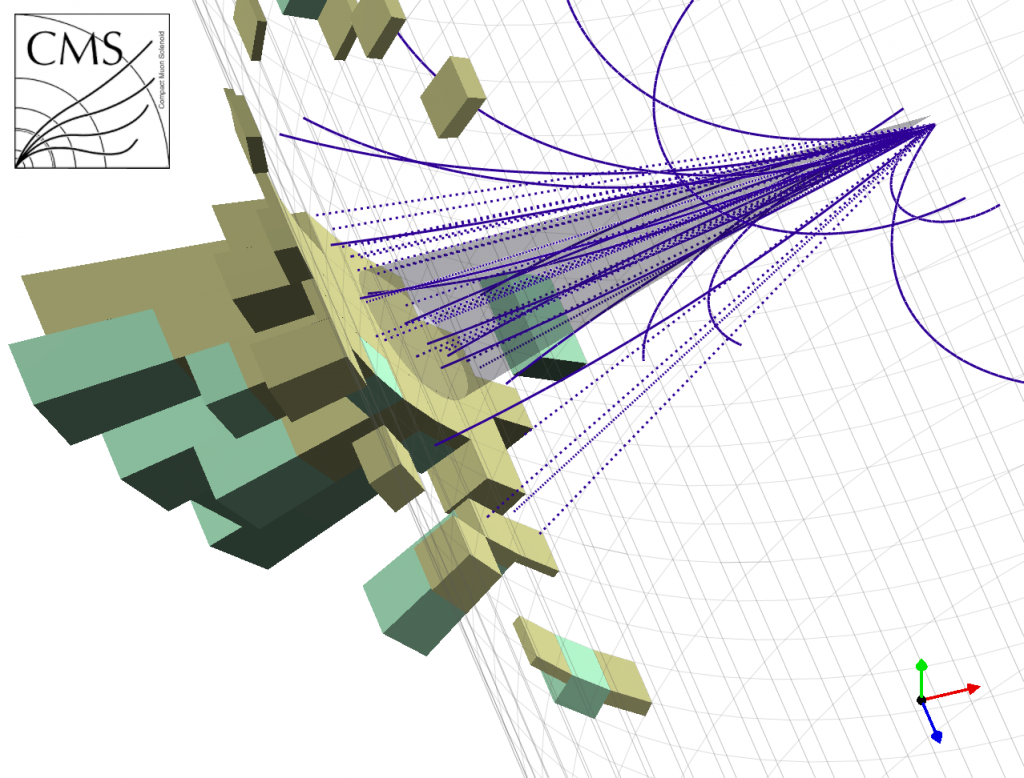
\includegraphics[width=0.75\textwidth]{figures/jetClusteringInCMS.png}
	\caption{A cone of reconstructed particles clustered into a jet, with the reconstructed vertex on the right.  
	From the CMS Experiment.}
	\label{fig:jetClustering}
\end{figure}

The high instantaneous luminosity of pp collisions delivered by the LHC almost always resulted in collision events with 
multiple reconstructed vertices, which represented pileup interactions.  The dominant effect of pileup interactions was 
the production of additional quarks and gluons, and thus additional jets.  Pileup jets originating from charged hadrons 
were significantly reduced by excluding charged hadrons from jet reconstruction that were not associated with the vertex, 
the primary vertex, that had the highest $\sum \pt$ in the event.  Neutral hadrons produced by pileup interactions contributed 
to the energies of all reconstructed jets, in addition to creating new jets.  Their effect was reduced by measuring the average 
neutral hadron energy density, $\rho$, over all $(\eta,\phi)$ in each event, and reducing the energy of jets reconstructed in each 
event by $\rho$ multiplied by each jet's area \cite{pileup1,pileup2}.

In each collision event, every reconstructed particle was considered a jet candidate except the charged hadrons from pileup 
vertices.  Candidate particles were clustered into jets using the anti-$k_{T}$ algorithm \cite{antikt} to cluster particles 
based on their $\pt$ and distance $\Delta R$ from the jet axis.  The jet axis was defined initially by a charged hadron, and 
was updated iteratively based on the $\pt$ weighted $(\eta,\phi)$ trajectories of all jet constituents.  Jets were built 
from particles reconstructed anywhere in the detector, but the anti-$k_{T}$ algorithm used a cone size of $\Delta R = 0.4$ to reduce the 
likelihood of having a jet constituent that was $\Delta R > 0.4$ away from the jet axis.  Once a jet was clustered its 
energy was determined as the $\sum \pt$ of all jet constituents.  Reconstructing jets from individual particles benefitted 
from the energy resolution of the tracker and the ECAL, and as a result jets with $\pt > 50$ $\GeV$ and $|\eta| < 3.0$ were 
measured with $\pt$ resolution better than 15\% \cite{jetResolutionInCollisions}.

The energies of reconstructed jets were corrected based on several observed effects.  As described previously, neutral 
hadrons produced in pileup interactions contributed to the energies of all jets, and their contributions were mitigated by 
reducing each jet's energy based on its $(\eta,\phi)$ area.  Following this subtraction, jets reconstructed in dijet, $Z$+jet, 
or $\gamma$+jet events were used to match the jet energy scale and resolution in data and simulations used to estimate the 
signal and backgrounds.  In simulated events jets were found to have a different energy scale and resolution, and these 
differences were resolved by correcting jet energies in data and simulated events, using methods described elsewhere \cite{jetpaper}.  


\section{Conclusion}
\label{sec:recoConclusion}
Energetic electrons, muons and jets produced in collisions were reconstructed using several CMS sub-detectors and high energy 
reconstruction algorithms.  Additional selections were applied to reconstructed leptons and jets to increase sensitivity to the \WR 
signal relative to ST backgrounds that produced $\ell\ell jj$ events.

%%%%%%%%%%%%%%%%%%%%%%%%%%%%%%%%%%%%%%%%%%%%%%%%%%%%%%%%%%%%%%%%%%%%%%%%%%%%%%%%
